
\section{System Model}
\label{sec:model}

In this section, we present our model for transactions, invariants,
and coordination.

\minihead{Transactions} In this paper, we consider a set of users
accessing a shared database, which contains a versioned set of data
items. In our initial formulation, we will represent database state as
a bag of mutations (much like a write-ahead log~\cite{gray-book}), but
we will consider other, more pragmatic representations in
Section~\ref{sec:bcc-practice}; we assume that the database is
initially populated by an initial state $D_0$ (typically but not
necessarily empty). Users submit requests to the database in the form
of transactions, or groups of operations on data items that should be
executed together. Operations are often in the form of writes (which
add a new version to the database) or reads (which return a specific
version--or set of versions--from the database), but operations can
also operate on abstract data types, such as incrementing a counter
item or adding an item to a set item. When required---and certainly in
future sections of this paper---we will discuss specific operation
types, but, in general, we will not make any specific assumptions
about operations. A transaction can \textit{commit}, signaling
success, or \textit{abort}, signaling failure. As a pragmatic
guarantee (not strictly required for our formalism), we will require
that no transaction that commits observes the effects of aborted
transactions, and, if a transaction commits, its effects should
survive database failures. We define a transaction $T$ as a
transformation on state with side effects: $T: DB \rightarrow DB$.

\minihead{Invariants} We consider a model where users specify
invariants over arbitrary database state that determine whether a
given state is valid. For example, an invariant might express the
requirement that only one user in a database has a given ID.  We model
invariants as binary predicates on database state: $I: DB \rightarrow
\{true, false\}$. Given a set of invariants $I_s$, we say that the
database is \textit{valid} under $I_s$ if all invariants in $I_s$
evaluate to true and w require that $D_0$ be valid. Invariants
directly capture the notion of ACID
Consistency~\cite{bernstein-book,gray-virtues}.

\miniheadnostop{Why specify invariants?} The majority of existing work
on database concurrency control assumes a model whereby ``the [set of
  invariants] is generally not known to the system but is embodied in
the structure of the transaction''~\cite{traiger-tods}. Indeed,
Eswaran et al.'s seminal paper on the topic of consistency argues that
``a complete set of assertions would no doubt be as large as the
system istself''~\cite{eswaran-consistency}. Nevertheless, since 1976,
databases have introduced support for a finite set of
invariants~\cite{korth-serializability} in the form of primary key and
foreign key, uniqueness, and row-level ``check'' constraints. We
expand this set of invariants in Section~\ref{sec:bcc-practice} and
demonstrate that a small set of invariants adds sufficient expressive
power for many applications. It is possible to perform a conservative
analysis if a complete specification of invariants is missing, but
this will result in less useful results. One consolation is that,
unlike more general forms of axiomatic logic (e.g., Hoare-style
triples~\cite{decomp-semantics}), there is only one (set of)
invariant(s) defined per application that is applied for every
transaction.\vspace{.5em}

\minihead{Coordination} In this paper, we are concerned with
synchronization and coordination between multiple transactions. We
consider a system model with are multiple, replicated copies of
database state (\textit{replicas}) located in separate processes
(\textit{servers}) that can each respond to transaction requests.  To
prevent the system from unnecessarily aborting transactions in order
to provide a response, we say that a system provides
\textit{transactional availability} (liveness) if, whenever a client
executing a transaction $T$ can access at least one replica for each
item in $T$, $T$ eventually commits or otherwise aborts itself either
due to an \textit{abort} operation in $T$ or due to a violation of a
declared integrity constraint~\cite{hat-vldb}.\footnote{As Bailis et
  al. note~\cite{hat-vldb}, this definition precludes multi-server
  fault tolerance (durability). However, we can consider multi-server
  durability by extending this definition to include coordination with
  a finite number of servers. This does not greatly affect scalability
  because, as more replicas are added, coordination is constant.} We
say that a system is \textit{always valid} if all replicas always
contain valid state. To capture the effect of network partitions but
also to capture linear scalability, we say that a system is
\textit{\cfree} if replicas do not communicate in order to execute
transactions.

It is vacuously possible to maintain ``consistent'' database states by
letting replicas diverge: in distributed systems parlance, this
guarantees \textit{safety} but not
\textit{liveness}~\cite{lamport-safety}. To ensure that replicas
eventually agree---reflecting a shared, common set of database
state---we will say that a system is \textit{convergent} if, in the
absence of new transactions and in the absence of indefinite
communication delays, all replicas eventually contain the same state
(i.e., via \textit{anti-entropy} processes)~\cite{vogels-defs}. To
capture the process of reconciling divergent copies of database state,
we introduce a \textit{merge} operator (denoted $\sqcup$) that, given
two copies of database state, produces a single copy of database state
representing the two divergent states. For our initial presentation,
our merge operator will be simple set union, but we discuss
alternative merge operators in Section~\ref{sec:merge}. We make no
assumptions about merge except that it be commutative, associative,
and idempotent~\cite{calm,crdt}.

Figure~\ref{fig:replicas} depicts a coordination-free execution of two
transactions $T_1$ and $T_2$ on two separate replicas of (complete)
database state. Each transaction commits on its local replica, which
subsequently forwards the new database state to the other replica in
the background. By applying the merge operator of set union, each
replica contains the same database state.

\begin{figure}
\begin{center}
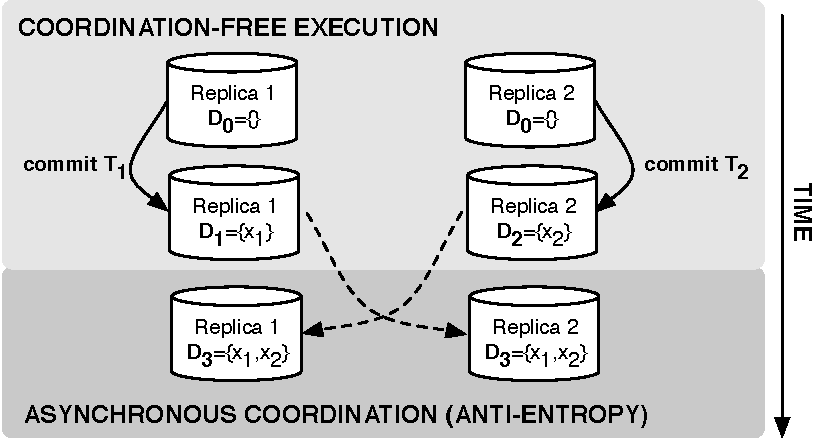
\includegraphics[width=.85\columnwidth]{figs/replicas.pdf}
\end{center}
\caption{An example coordination-free execution of two transactions,
  $T_1$ and $T_2$ on two replicas of database state. Each transaction
  commits on a replica, then, after commit, the replicas exchange
  their new writes asynchronously and converge on a common database
  state ($D_3$).}
\label{fig:replicas}
\end{figure}


\miniheadnostop{A note on replicas} While most treatments of
distributed databases (including this one) often treat replicas as
individual servers, even a non-replicated database can provide users
with an interface that exposes multiple ``replicas''. In fact, a
multi-versioned database system~\cite{bernstein-book} effectively
provides each user with a copy of database state, even in the presence
of concurrent access and modification. The specific concurrency
control mechanism will dictate which transactions commit or not, but a
set of invariants and stored procedures that are achievable without
coordination can also be executed in parallel on a single-site system
without aborts due to concurrent operations or other isolation
anomalies.  In fact, our current prototype transaction model
(Section~\ref{sec:evaluation}) is based on multi-versioning and
snapshot reads (``logical replicas'') rather than actual multi-master
replication. Similar analogies can be drawn to general-purpose
optimistic methods (but not as much to lock-based schemes, which
largely limit concurrency), although we do not consider them here.
